\documentclass[tikz,border=10pt]{standalone}
\usepackage{tikz}
\usetikzlibrary{shapes.geometric, arrows.meta, positioning, fit, backgrounds}

\begin{document}
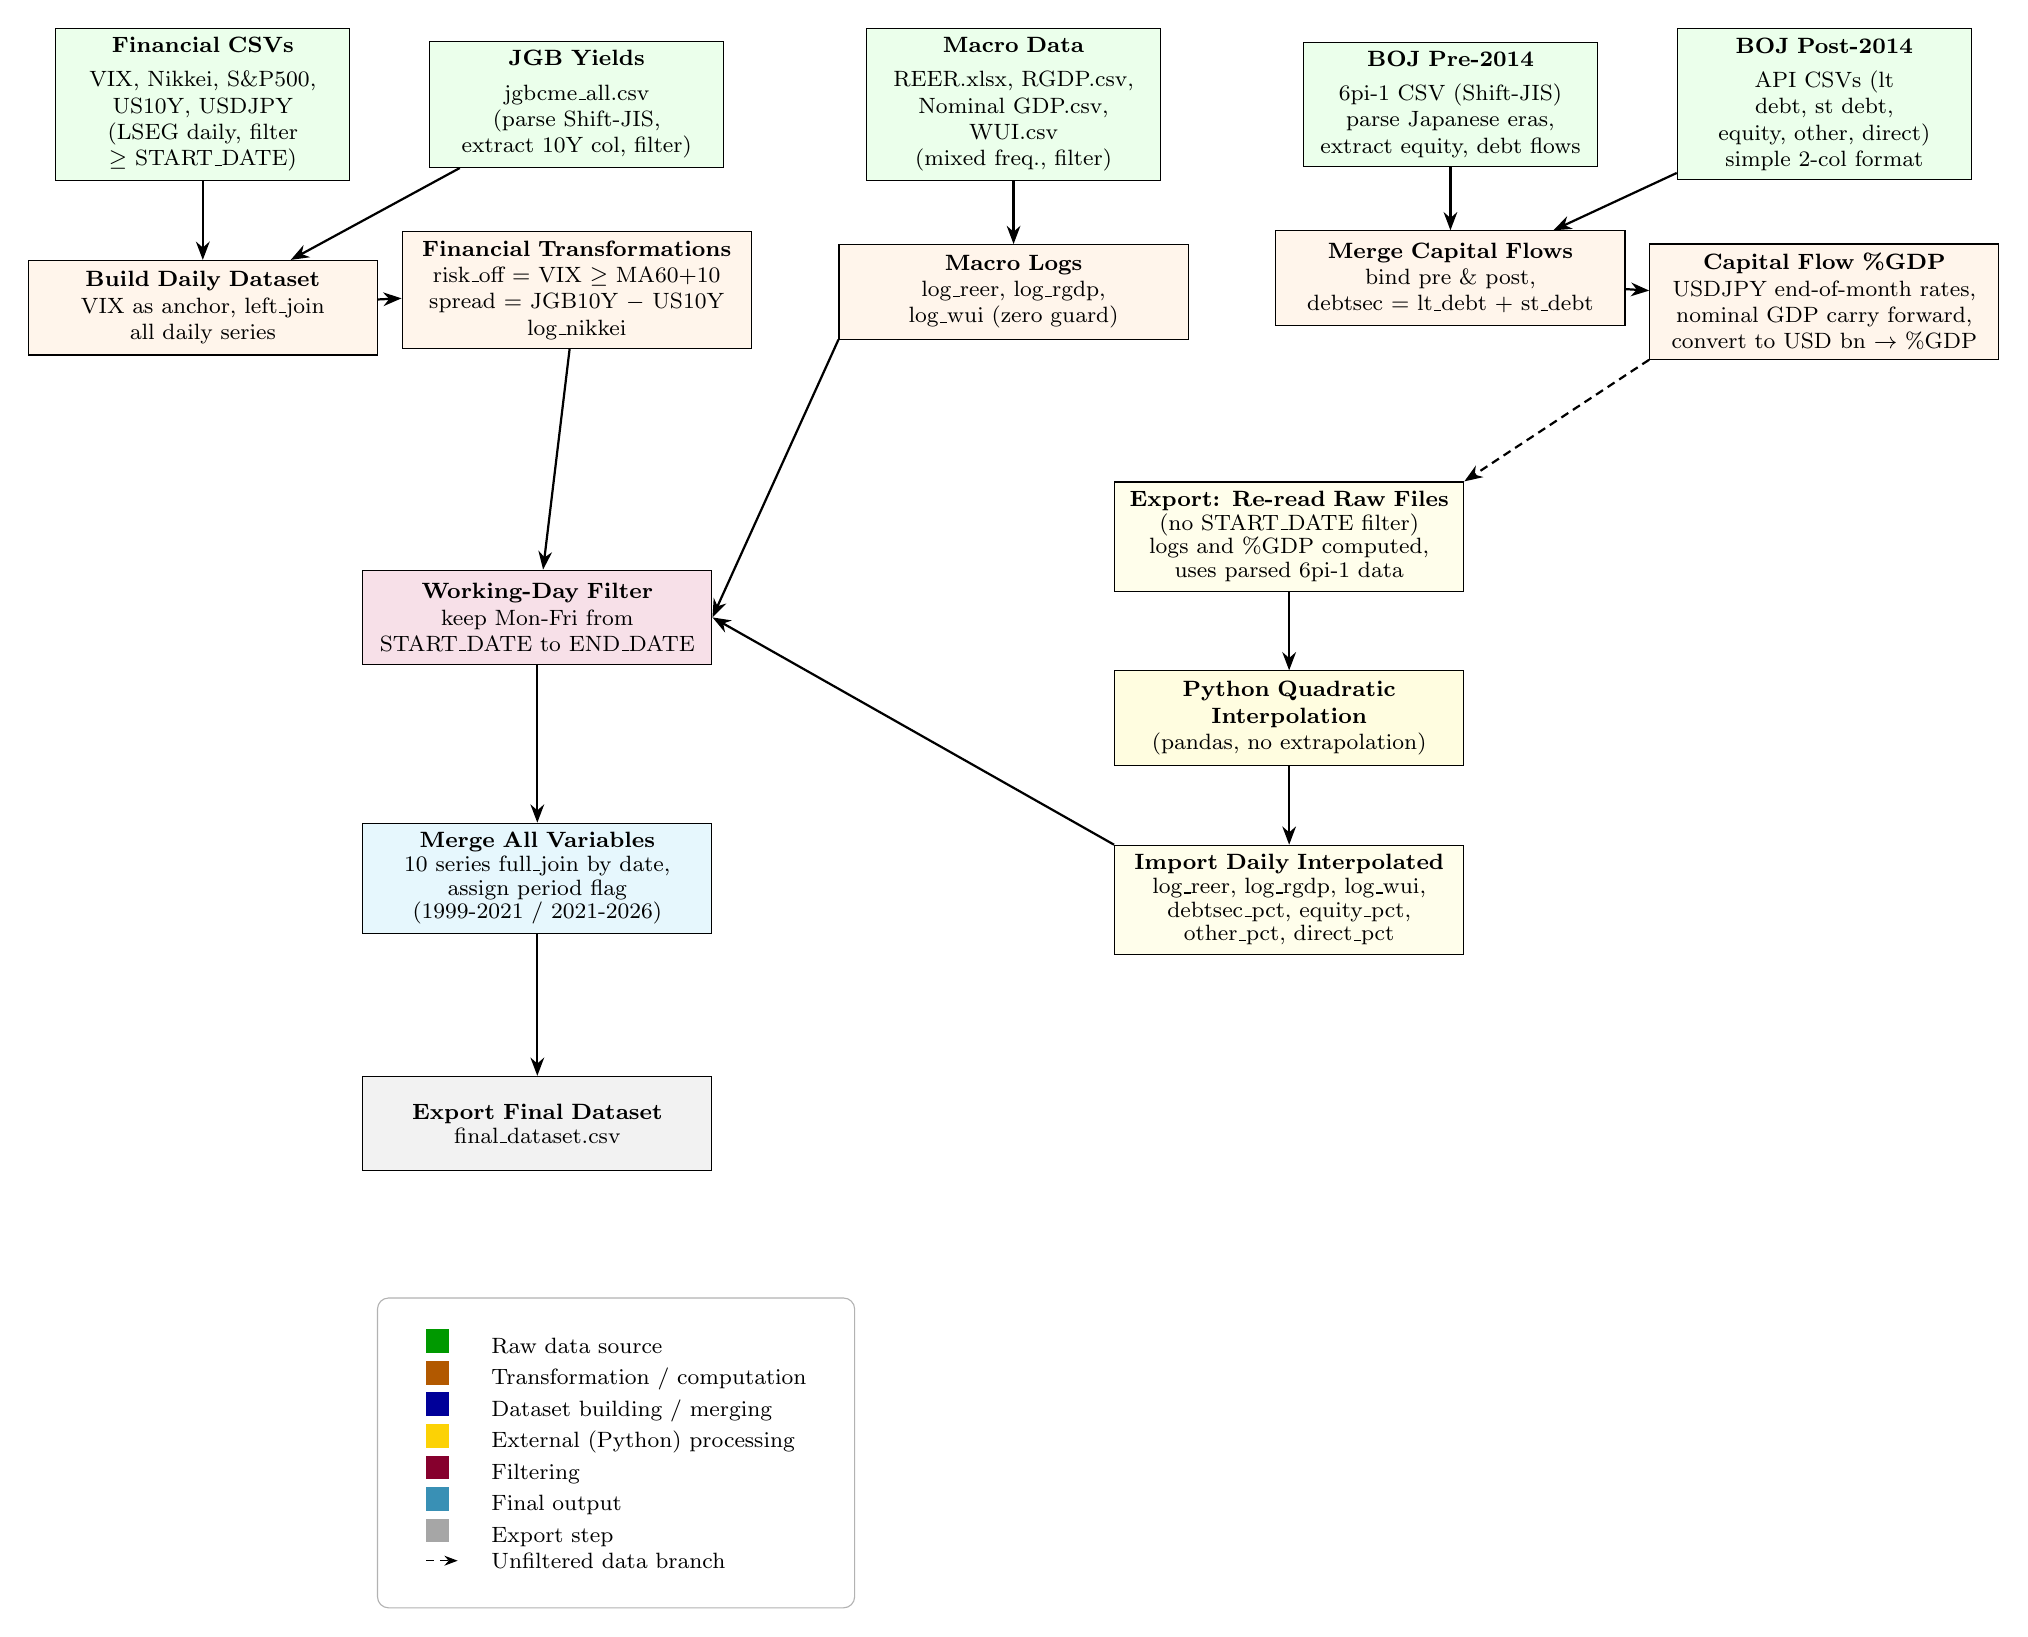
\begin{tikzpicture}[
  node distance = 8mm and 10mm,
  block/.style = {
    rectangle, draw, fill=blue!8,
    text width=4.2cm, align=center, minimum height=1.2cm,
    font=\footnotesize\linespread{0.9}\selectfont
  },
  smallblock/.style = {
    block, text width=3.8cm, minimum height=1cm
  },
  datasrc/.style = {
    rectangle, draw, fill=green!8,
    text width=3.5cm, align=center, minimum height=0.9cm,
    font=\footnotesize
  },
  proc/.style = {
    rectangle, draw, fill=orange!8,
    text width=4.2cm, align=center, minimum height=1.2cm,
    font=\footnotesize
  },
  branch/.style = {
    draw, densely dashed, ->, >=Stealth, thick
  },
  arrow/.style = {
    ->, >=Stealth, thick
  },
  label/.style = {
    font=\scriptsize\itshape
  }
]

% ====== DATA SOURCES (top row) ======
\node[datasrc] (fin) {
  \textbf{Financial CSVs}\\[1mm]
  VIX, Nikkei, S\&P500,\\
  US10Y, USDJPY\\
  (LSEG daily, filter \(\ge\) START\_DATE)
};

\node[datasrc, right=of fin] (jgb) {
  \textbf{JGB Yields}\\[1mm]
  jgbcme\_all.csv\\
  (parse Shift-JIS,\\
  extract 10Y col, filter)
};

\node[datasrc, right=of jgb, xshift=8mm] (macro) {
  \textbf{Macro Data}\\[1mm]
  REER.xlsx, RGDP.csv,\\
  Nominal GDP.csv, WUI.csv\\
  (mixed freq., filter)
};

\node[datasrc, right=of macro, xshift=8mm] (bojpre) {
  \textbf{BOJ Pre-2014}\\[1mm]
  6pi-1 CSV (Shift-JIS)\\
  parse Japanese eras,\\
  extract equity, debt flows
};

\node[datasrc, right=of bojpre] (bojpost) {
  \textbf{BOJ Post-2014}\\[1mm]
  API CSVs (lt debt, st debt,\\
  equity, other, direct)\\
  simple 2-col format
};

% ====== MERGE / AGGREGATE (row 2) ======
\node[proc, below=of fin, yshift=-2mm] (dailybuild) {
  \textbf{Build Daily Dataset}\\
  VIX as anchor, left\_join\\
  all daily series
};

\node[proc, below=of jgb] (derivedfin) {
  \textbf{Financial Transformations}\\
  risk\_off = VIX \(\ge\) MA60+10\\
  spread = JGB10Y $-$ US10Y\\
  log\_nikkei
};

\node[proc, below=of macro] (macrolog) {
  \textbf{Macro Logs}\\
  log\_reer, log\_rgdp,\\
  log\_wui (zero guard)
};

\node[proc, below=of bojpre] (mergeflows) {
  \textbf{Merge Capital Flows}\\
  bind pre \& post,\\
  debtsec = lt\_debt + st\_debt
};

\node[proc, below=of bojpost] (pctgdp) {
  \textbf{Capital Flow \%GDP}\\
  USDJPY end-of-month rates,\\
  nominal GDP carry forward,\\
  convert to USD bn \(\to\) \%GDP
};

% ====== UNFILTERED BRANCH (row 3-5, shifted 35mm right) ======
\node[block, fill=yellow!8,
      below=of macrolog, yshift=-10mm,
      xshift=35mm] (native) {
  \textbf{Export: Re-read Raw Files}\\
  (no START\_DATE filter)\\
  logs and \%GDP computed,\\
  uses parsed 6pi-1 data
};

\node[proc, fill=yellow!12, below=of native, yshift=-2mm] (python) {
  \textbf{Python Quadratic}\\
  \textbf{Interpolation}\\
  (pandas, no extrapolation)
};

\node[block, fill=yellow!8, below=of python, yshift=-2mm] (importd) {
  \textbf{Import Daily Interpolated}\\
  log\_reer, log\_rgdp, log\_wui,\\
  debtsec\_pct, equity\_pct,\\
  other\_pct, direct\_pct
};

% ====== WORKING-DAY FILTER (row 4) ======
\node[proc, fill=purple!12,
      below=of derivedfin, yshift=-20mm,
      xshift=-5mm] (workday) {
  \textbf{Working-Day Filter}\\
  keep Mon-Fri from\\
  START\_DATE to END\_DATE
};

% ====== FINAL MERGE & EXPORT (row 5) ======
\node[block, fill=cyan!10,
      below=of workday, yshift=-12mm] (final) {
  \textbf{Merge All Variables}\\
  10 series full\_join by date,\\
  assign period flag\\
  (1999-2021 / 2021-2026)
};

\node[block, fill=gray!10,
      below=of final, yshift=-10mm] (export) {
  \textbf{Export Final Dataset}\\
  final\_dataset.csv
};

% ====== ARROWS ======
% Financial sources -> daily build
\draw[arrow] (fin) -- (dailybuild);
\draw[arrow] (jgb) -- (dailybuild);
\draw[arrow] (dailybuild) -- (derivedfin);

% Macro -> macro logs
\draw[arrow] (macro) -- (macrolog);

% BOJ -> merge flows
\draw[arrow] (bojpre) -- (mergeflows);
\draw[arrow] (bojpost) -- (mergeflows);
\draw[arrow] (mergeflows) -- (pctgdp);

% ** THE FIX: Dashed arrow from Capital Flow %GDP to the Export step **
\draw[branch] (pctgdp.south west) -- (native.north east);

% Unfiltered branch: re-reads raw files + parses
\draw[arrow] (native) -- (python);
\draw[arrow] (python) -- (importd);

% Working-day -> final -> export

% Financial outputs and interpolated series -> working-day filter
\draw[arrow] (derivedfin) -- (workday);
\draw[arrow] (macrolog.south west) -- (workday.east);
\draw[arrow] (importd.north west) -- (workday.east);

% Working-day -> final -> export
\draw[arrow] (workday) -- (final);
\draw[arrow] (final) -- (export);

% ---- background legend ----
\begin{scope}[on background layer]
\node[draw=gray!60, fill=white, rounded corners,
      font=\footnotesize, inner sep=4mm,
      below=of export, yshift=-8mm,
      xshift=10mm, anchor=north] (legend) {
  \begin{tabular}{ll}
    {\color{green!60!black}\rule{3mm}{3mm}} & Raw data source \\
    {\color{orange!70!black}\rule{3mm}{3mm}} & Transformation / computation \\
    {\color{blue!60!black}\rule{3mm}{3mm}} & Dataset building / merging \\
    {\color{yellow!70!orange}\rule{3mm}{3mm}} & External (Python) processing \\
    {\color{purple!70!black}\rule{3mm}{3mm}} & Filtering \\
    {\color{cyan!70!black}\rule{3mm}{3mm}} & Final output \\
    {\color{gray!70}\rule{3mm}{3mm}} & Export step \\
    \raisebox{1pt}{\tikz{\draw[densely dashed,->,>=Stealth] (0,0) -- (0.4,0);}} & Unfiltered data branch
  \end{tabular}
};
\end{scope}

\end{tikzpicture}
\end{document}